% FIGURES
% Fig 1
\begin{figure*}
    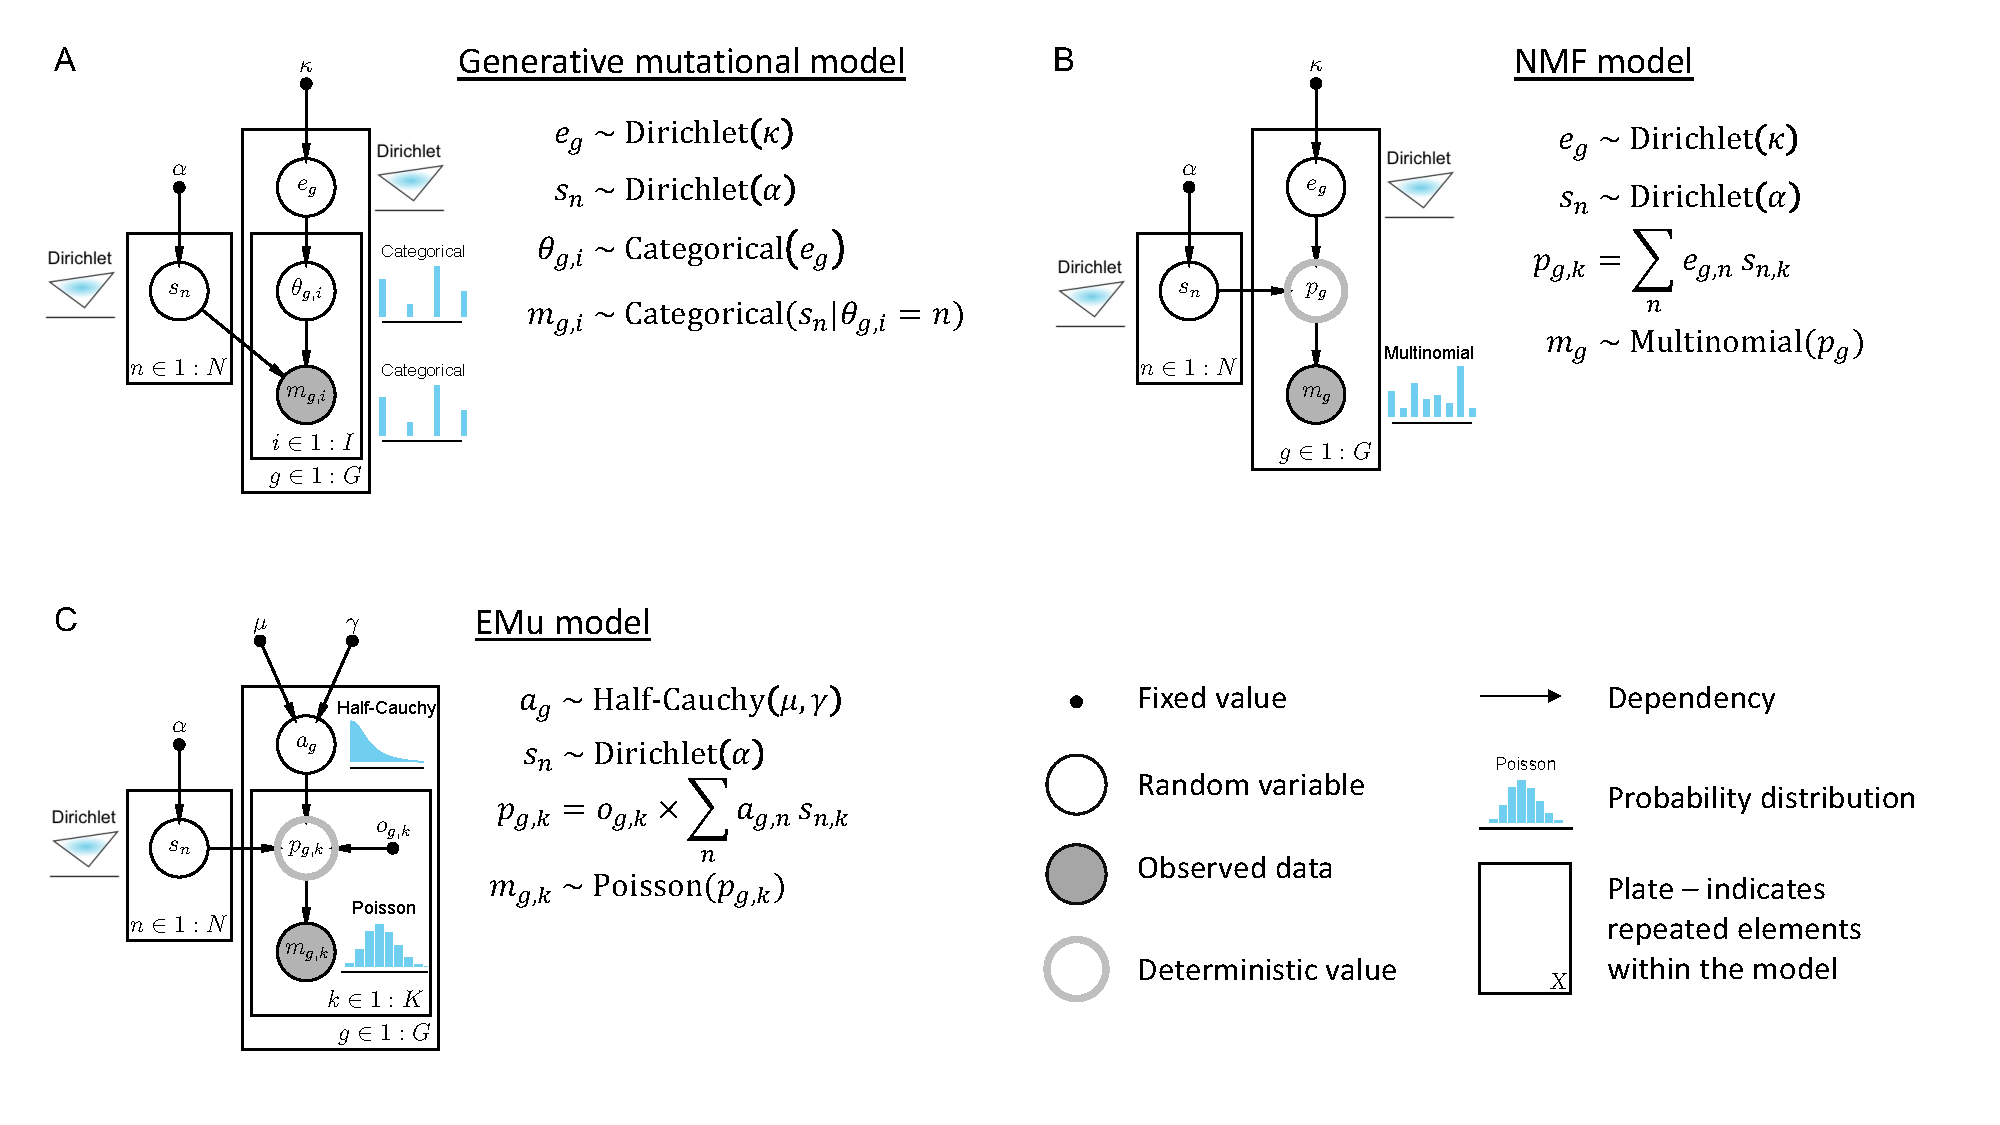
\includegraphics[width=\textwidth]{Figure1_v9.pdf}
    \caption[Figure 1]{\textbf{Bayesian model diagrams. (A)} A generative model of mutation with multiple mutational processes. Each mutational catalogue (indexed by $g$) accumulates $I$ mutations. Each mutation ${m_{g,i}}$ is produced by mutational process $n$ of $N$ processes. $\theta_{g, i}$ encodes the choice of mutational process for mutation ${m_{g,i}}$ in catalogue $g$. $\theta$ is assigned by a draw from a categorical distribution, parameterised by probabilities $e_{g}$, which are in turn drawn from a Dirichlet distribution parameterised by $\kappa$. The type of mutation is chosen by drawing from a categorical distribution, parameterised by probabilities $s_{n}$, in turn drawn from a Dirichlet distribution parameterised by $\alpha$. \textbf{(B)} The NMF-inspired inferential model is based on the generative model, with the distinction that, as the allocation of individual mutations to specific processes is not of interest, the latent parameter $\theta$ is marginalised out. The process of marginalisation is to matrix-multiply the exposures ($E$, where $e_{g}$ is the $g$-th row) and the signatures ($S$, where $s_{n}$ is the $n$-th row), to yield a matrix of probabilities ($P$, where $p_{g}$ is the $g$-th row). $P$ is denoted by a node with a grey outline to indicate that it is a deterministic value, to distinguish it from random variable nodes, which take a black outline. The likelihood of the observed mutational catalogue $m_g$ is obtained from the probability mass function of a multinomial distribution parameterised by $p_g$. \textbf{(C)} The EMu-inspired inferential model differs from the NMF-inspired model in that the mutation counts per mutation category, $m_{g,k}$, are modelled as if generated by a Poisson distribution, parameterised by the matrix product of the activities ($A$) and the signatures ($S$), element-wise multiplied by the opportunities matrix ($O$). A half-Cauchy distribution is used as the choice of prior for $A$, as the activities are not required to sum to unity. Plate notation diagrams were produced using daft-pgm (\url{http://daft-pgm.org/})}.
    \label{figure1}
\end{figure*}

% Figure 2
\begin{figure*}
    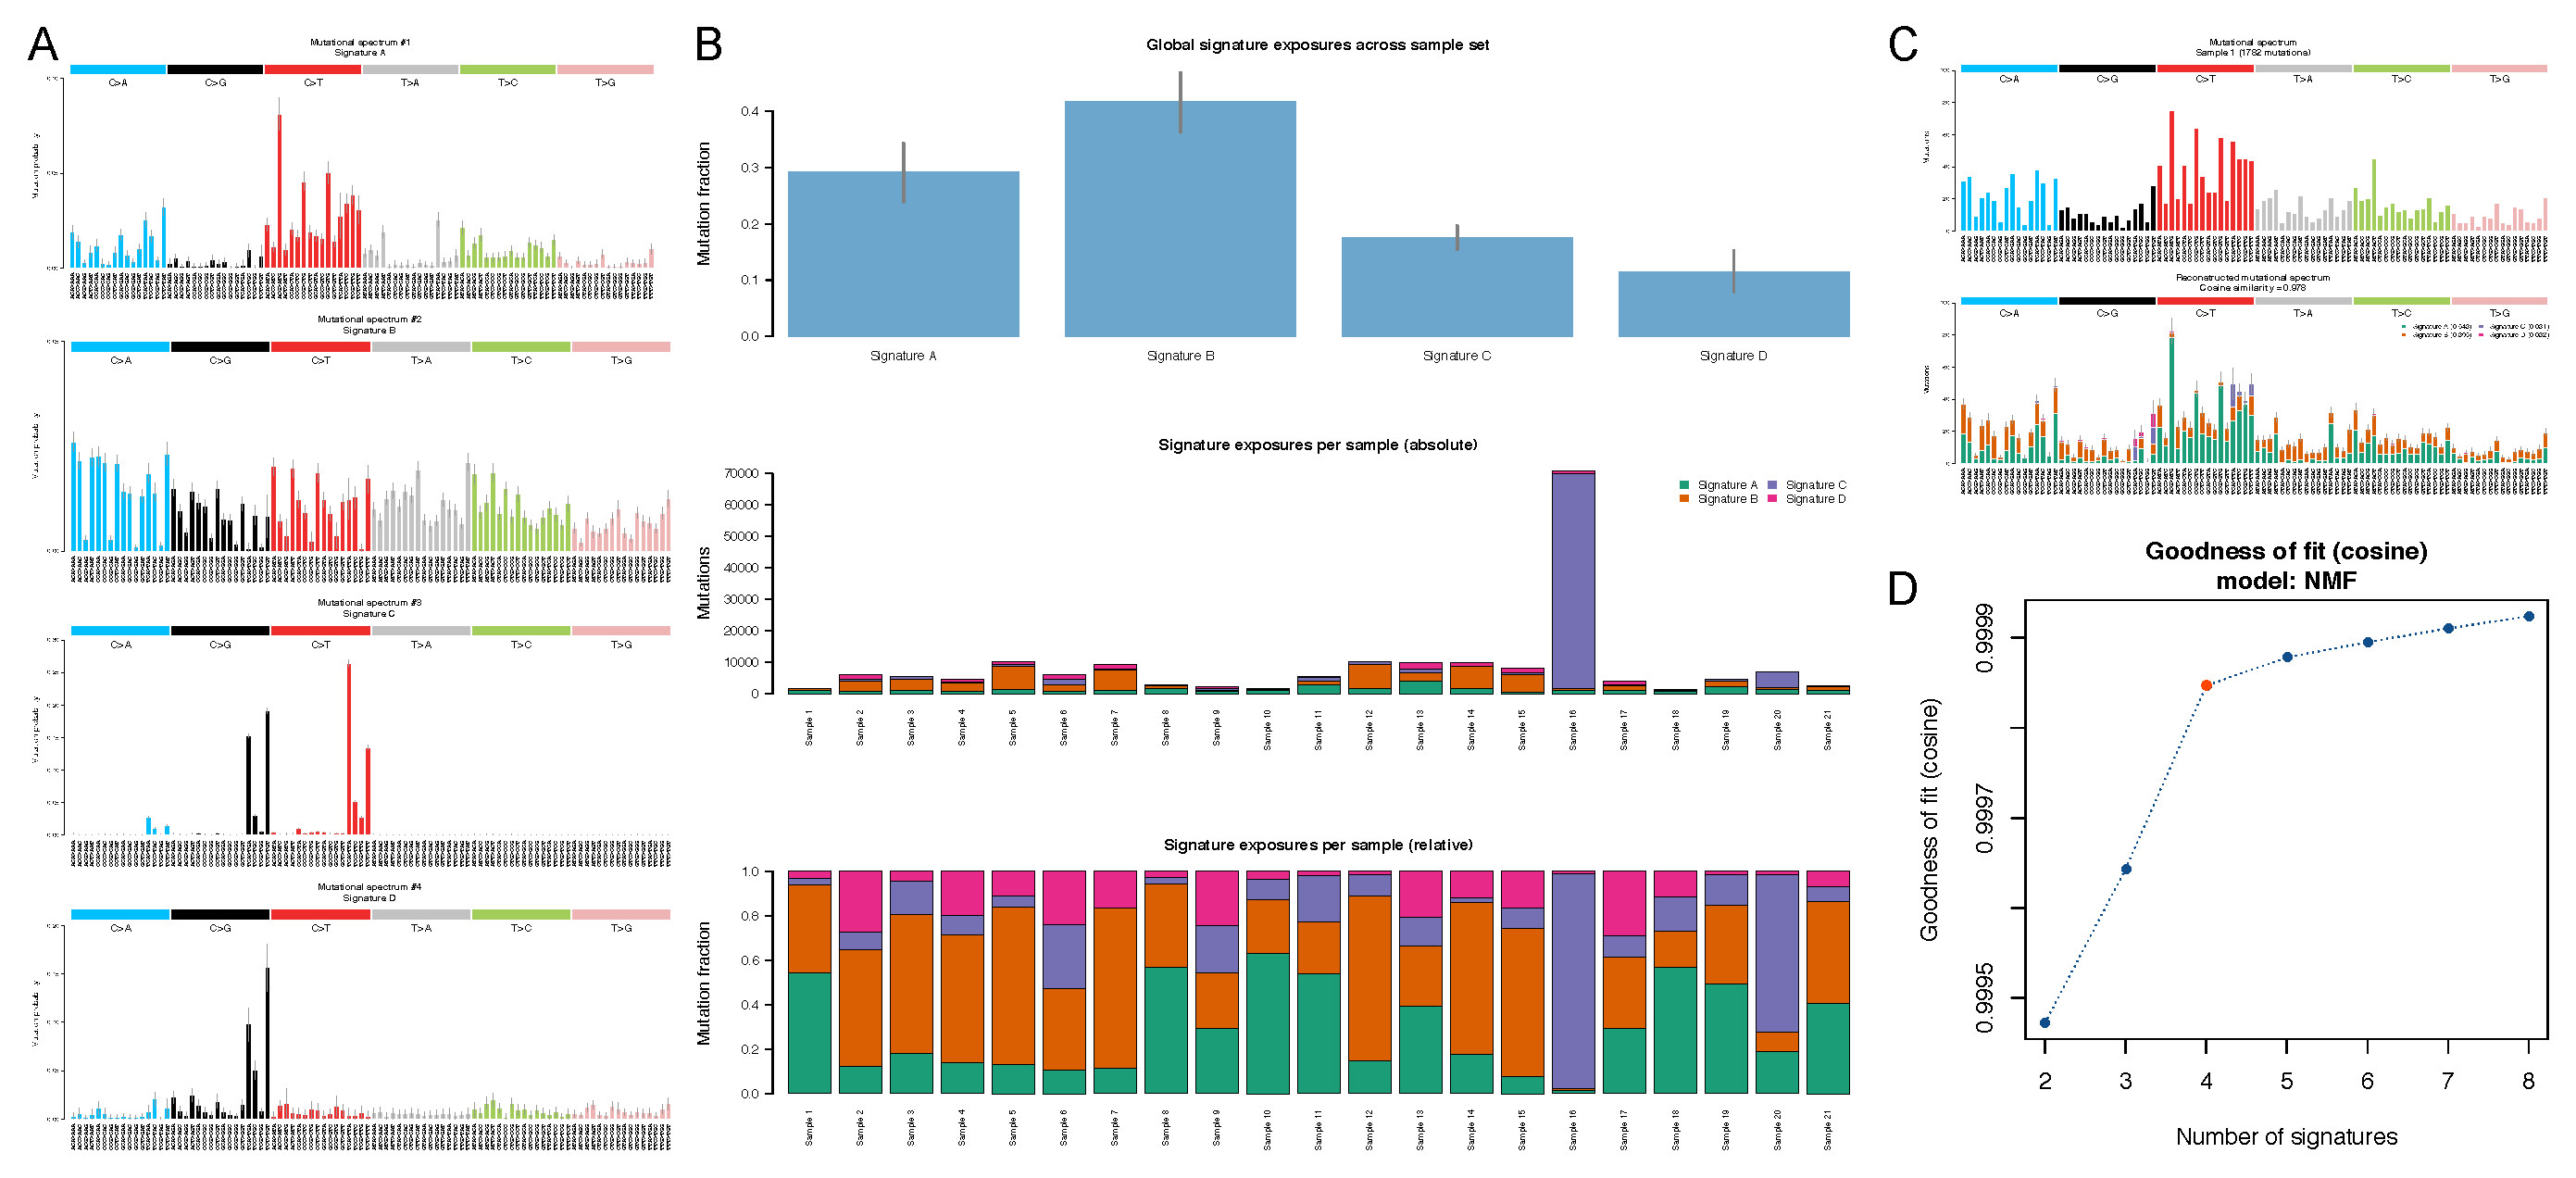
\includegraphics[width=\textwidth]{Figure2_v2.pdf}
    \caption[Figure 2]{\textbf{Plotting capabilities of sigfit.} The plots in panels (A–C) were produced using the `plot\_all' function in sigfit, from the results obtained by extracting four signatures from a set of 21 breast cancer catalogues \citep{Nik-Zainal2012:mp21bc}. \textbf{(A)} The four signatures extracted by sigfit; the most similar signatures in COSMIC are signatures 1, 3, 2 and 13, respectively. \textbf{(B)} Signature exposures across the set of catalogues as a whole (top), and within each catalogue, both as absolute mutation counts (middle) and in relation to the total number of mutations (bottom). \textbf{(C)} Plot of the reconstruction of an example mutational catalogue from the estimated signatures and exposures. The original catalogue is shown above the reconstructed one. \textbf{(D)} Evaluation of the reconstruction accuracy for a range of numbers of signatures, plotted using the `plot\_gof' function in sigfit. A value of four signatures is automatically suggested as the point maximising the approximated second derivative of the curve (indicated in orange).}
    \label{figure2}
\end{figure*}

% Fig 3
\begin{figure*}
    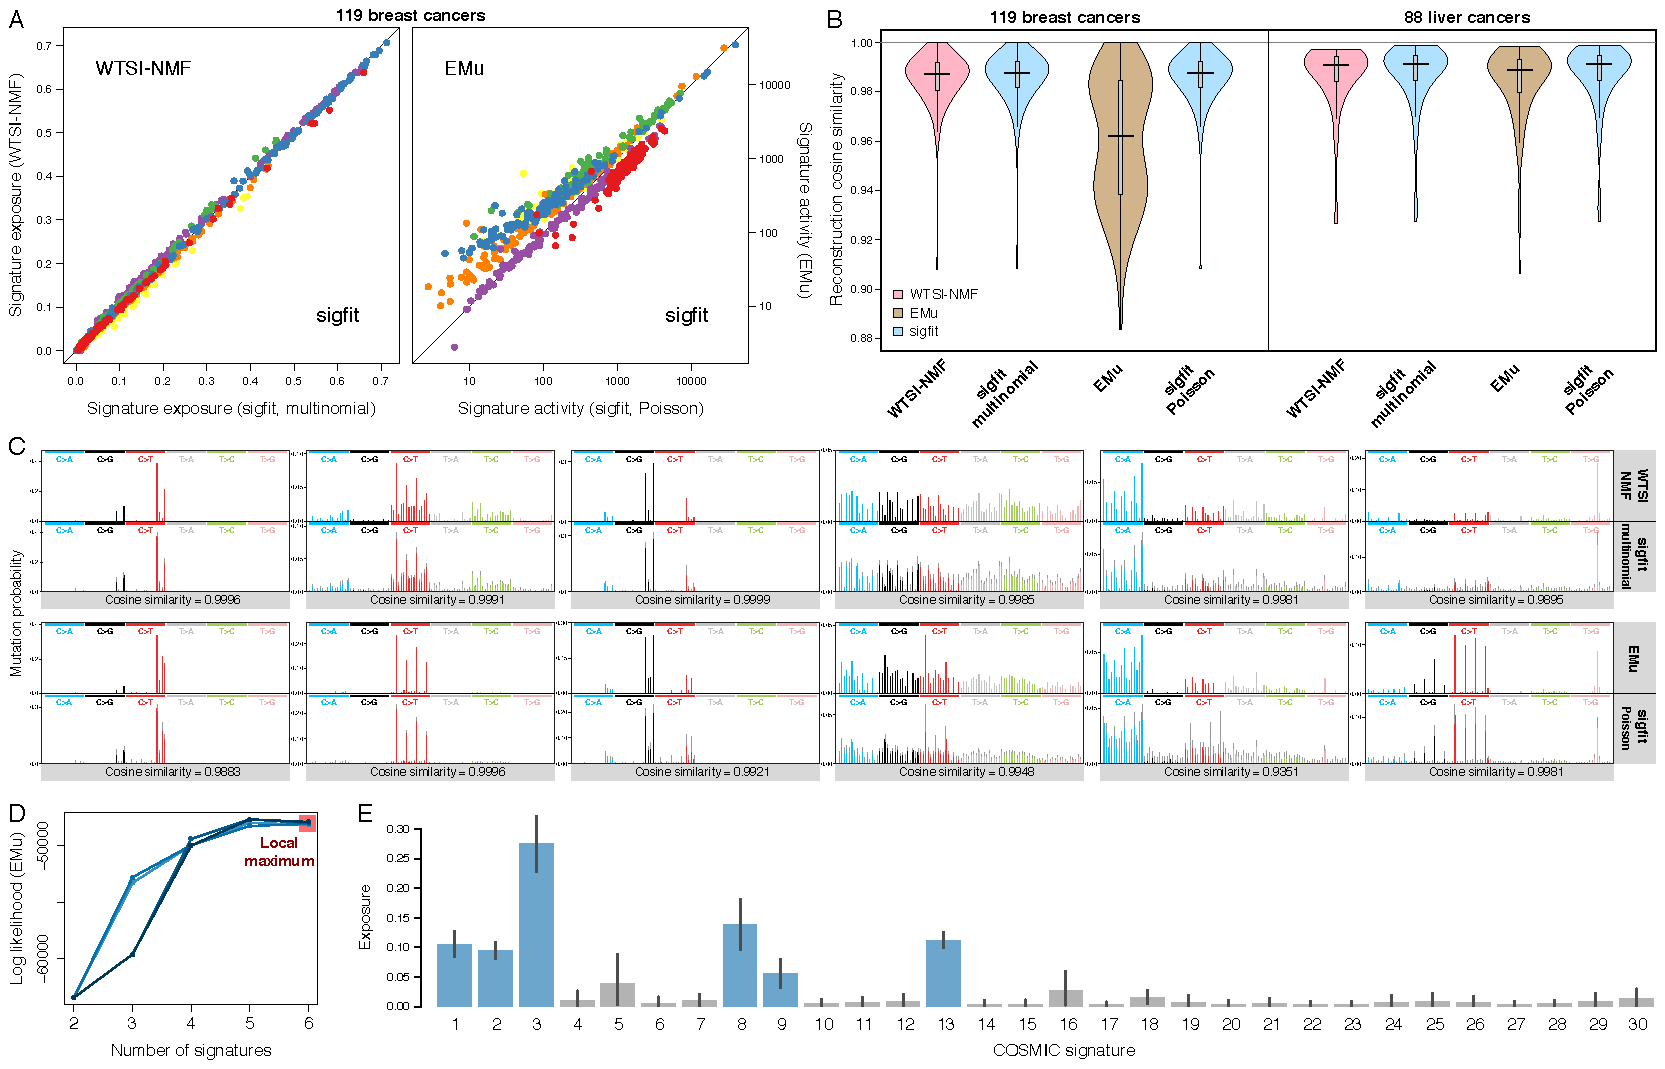
\includegraphics[width=\textwidth]{Figure3_v4}
    \caption[Figure 3]{\textbf{Evaluation of the performance of sigfit models for signature extraction and fitting. (A)} Left, comparison of signature exposures (proportion of mutations attributed to each signature) as estimated by the Dirichlet–Multinomial model in sigfit (horizontal axis) and the WTSI-NMF software (vertical axis). Right, comparison of signature activities (number of mutations attributed to each signature) as estimated by the Poisson model in sigfit (horizontal axis) and the EMu software (vertical axis). The results correspond to extraction of six mutational signatures from a set of 119 breast cancer mutational catalogues \cite{Alexandrov2013}. Dot colours distinguish between the six mutational signatures. \textbf{(B)} Distributions of reconstruction accuracy (cosine similarity between the original and reconstructed catalogues) for the models in sigfit and the WTSI-NMF and EMu software, in a set of 119 breast cancer catalogues (left) and a set of 88 liver cancer catalogues (right) \cite{Alexandrov2013}. Boxplots are shown within each violin plot, and horizontal lines indicate median cosine similarity. Violin colours distinguish between software tools. \textbf{(C)} Comparison of mutational signatures extracted \textit{de novo} by WTSI-NMF and the Dirichlet–Multinomial model in sigfit (top row), and by EMu and the Poisson model in sigfit (bottom row) from a set of 119 breast cancer catalogues \cite{Alexandrov2013}. Cosine similarity between analogous pairs of signatures is shown below each. Vertical axes present mutation probabilities, and bars represent 96 trinucleotide mutation types (see main text), with colours indicating base substitution type. \textbf{(D)} Likelihood obtained by EMu over a range of numbers of signatures, for five different runs of the software. The decrease in likelihood when extracting six signatures (highlighted in red) indicates convergence of the EM algorithm to a local maximum. \textbf{(E)} Posterior mean estimates of global signature exposures inferred by the Dirichlet–Multinomial signature fitting model in sigfit, through fitting of the 30 signatures in COSMIC to a set of 21 breast cancer catalogues \cite{Nik-Zainal2012:mp21bc}. Error bars indicate 95\% highest posterior density (HPD) intervals. Grey bars indicate non-significant signature exposures, defined as exposures for which the lower end of the 95\% HPD interval is below 0.01.}
    \label{figure3}
\end{figure*}

% Fig 3
\begin{figure*}
    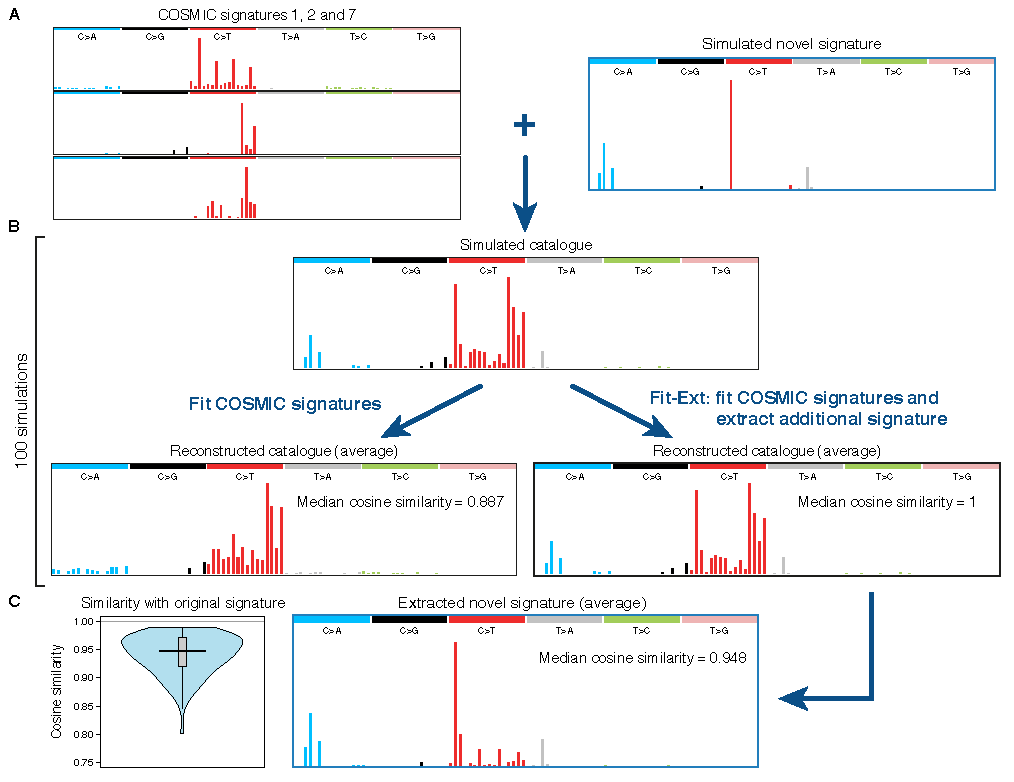
\includegraphics[width=\textwidth]{Figure4_v1.pdf}
    \caption[Figure 4]{\textbf{Evaluation of the Fit-Ext model on simulated mutation data. (A)} Mutational spectra of the three COSMIC signatures (left) and the simulated novel mutational signature (right) that were used to produce simulated mutational catalogues. \textbf{(B)} In each of 100 simulations, a mutational catalogue (top) was generated from a random mixture of the signatures shown in (A), and signature analysis was performed with sigfit via two separate approaches: using the Dirichlet–Multinomial fitting model to fit all COSMIC signatures to the catalogue (bottom left), and using the Dirichlet–Multinomial Fit-Ext model to fit all COSMIC signatures and extract one additional signature (bottom right). Average reconstructed mutational catalogues (constructed from the product of signatures and inferred exposures) and median cosine similarities between the original and reconstructed catalogues across all simulations, are shown for each approach. \textbf{(C)} Average mutational spectrum of the estimated novel signature as extracted by the Fit-Ext model across all simulations. The violin plot (left) presents the distribution of the cosine similarity between the original novel signature, shown in (A), and the inferred signature across all simulations. A boxplot is shown within the violin plot, and the horizontal line indicates the median cosine similarity.}
    \label{figure4}
\end{figure*}
